\documentclass[margin=5mm]{standalone}
\usepackage{tikz}
\usetikzlibrary{shapes.geometric}

\begin{document}

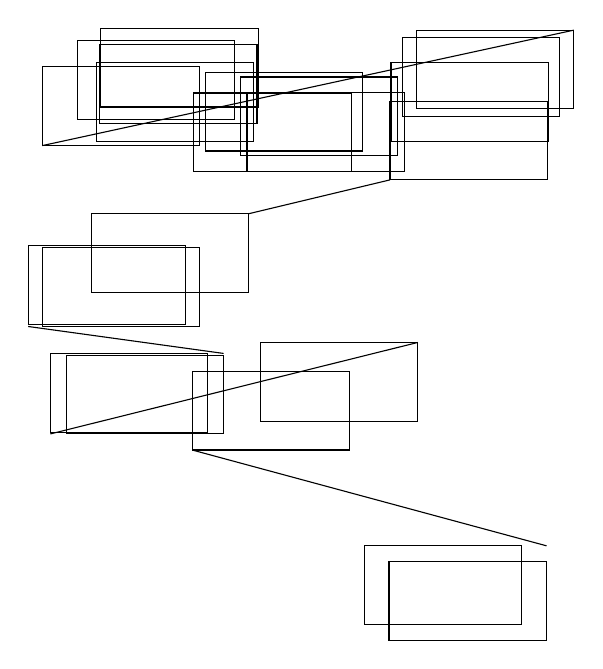
\begin{tikzpicture}[every node/.style={rectangle,minimum width=2cm,minimum height=1cm,draw}]

\begin{scope}[local bounding box=l]
\foreach \i in {0,...,4}{%
    \node (l\i) at (rnd,rnd){};}
\end{scope}

\begin{scope}[shift={(2,0)},local bounding box=m]
\foreach \i in {0,...,3}{%
    \node (m\i) at (rnd,rnd){};}
\end{scope}

\begin{scope}[shift={(4,0)},local bounding box=n]
\foreach \i in {0,...,3}{%
    \node (n\i) at (rnd,rnd){};}
\end{scope}


\begin{scope}[shift={(0,-2)},local bounding box=o]
\foreach \i in {0,...,2}{%
    \node (o\i) at (rnd,rnd){};}
\end{scope}

\begin{scope}[shift={(0,-4)},local bounding box=p]
\foreach \i in {0,...,1}{%
    \node (p\i) at (rnd,rnd){};}
\end{scope}

\begin{scope}[shift={(2,-4)},local bounding box=q]
\foreach \i in {0,...,1}{%
    \node (q\i) at (rnd,rnd){};}
\end{scope}


\begin{scope}[shift={(4,-6)},local bounding box=r]
\foreach \i in {0,...,1}{%
    \node (r\i) at (rnd,rnd){};}
\end{scope}


\draw (l.south west) -- (n.north east);
\draw (n.south west) -- (o.north east);
\draw (o.south west) -- (p.north east);
\draw (p.south west) -- (q.north east);
\draw (q.south west) -- (r.north east);

\end{tikzpicture}
\end{document}